\documentclass[10pt]{article}

\usepackage{fullpage}
\usepackage{amsmath}
\usepackage{amssymb}
\usepackage{amsthm}
\usepackage{fancyhdr}
\usepackage{algorithm}
\usepackage{algorithmic}
\usepackage{bm}
\usepackage{framed}
\usepackage{graphicx}
\usepackage{multirow}
\usepackage{hyperref}
\usepackage{natbib}
\usepackage[usenames,dvipsnames]{xcolor}


\newtheorem{theorem}{Theorem}[section]
\newtheorem{lemma}[theorem]{Lemma}
\newtheorem{corollary}[theorem]{Corollary}
\newtheorem{proposition}[theorem]{Proposition}
\newtheorem{definition}[theorem]{Definition}
\newtheorem{conjecture}[theorem]{Conjecture}
\newtheorem{remark}[subsection]{Remark}

%%
\newcommand\numberthis{\addtocounter{equation}{1}\tag{\theequation}}

%% define new symbols
\def\bx{\bm{x}}
\def\bb{\bm{b}}
\def\ba{\bm{a}}
\def\bc{\bm{c}}
\def\bf{\bm{f}}
\def\by{\bm{y}}
\def\bu{\bm{u}}
\def\bv{\bm{v}}
\def\BW{\bm{W}}
\def\BA{\bm{A}}
\def\bz{\bm{z}}
\def\BZ{\bm{Z}}
\def\BH{\bm{H}}
\def\BL{\bm{L}}
\def\BU{\bm{U}}
\def\BV{\bm{V}}
\def\BB{\bm{B}}
\def\BC{\bm{C}}
\def\BD{\bm{D}}
\def\BE{\bm{E}}
\def\BW{\bm{W}}
\def\BQ{\bm{Q}}
\def\BG{\bm{G}}
\def\BA{\bm{A}}
\def\BX{\bm{X}}
\def\BY{\bm{Y}}
\def\BQ{\bm{Q}}
\def\BI{\bm{I}}
\def\BR{\bm{R}}

%% define new brackets
\def\la{\left\langle}
\def\ra{\right\rangle}
\def\ln{\left\|}
\def\rn{\right\|}
\def\lb{\left(}
\def\rb{\right)}
\def\lsb{\left[}
\def\rsb{\right]}
\def\lcb{\left\{}
\def\rcb{\right\}}

%%
\DeclareMathOperator*{\argmin}{arg\,min}
\DeclareMathOperator*{\argmax}{arg\,max}

%%
\title{Project-1 Report of ``Neural Network and Deep Learning''}
\author{Jialun Shen\\ 16307110030}


\begin{document}
\maketitle
%------------------------------------
%\begin{abstract}
%\end{abstract}
%-------------------------------------
%=====================
\section{Neural Network}
\subsection{Questions}
\begin{enumerate}

\item Change the network structure: the vector \textit{nHidden} specifies the number of hidden units in each layer.

\begin{figure}[htbp]
  \centering
  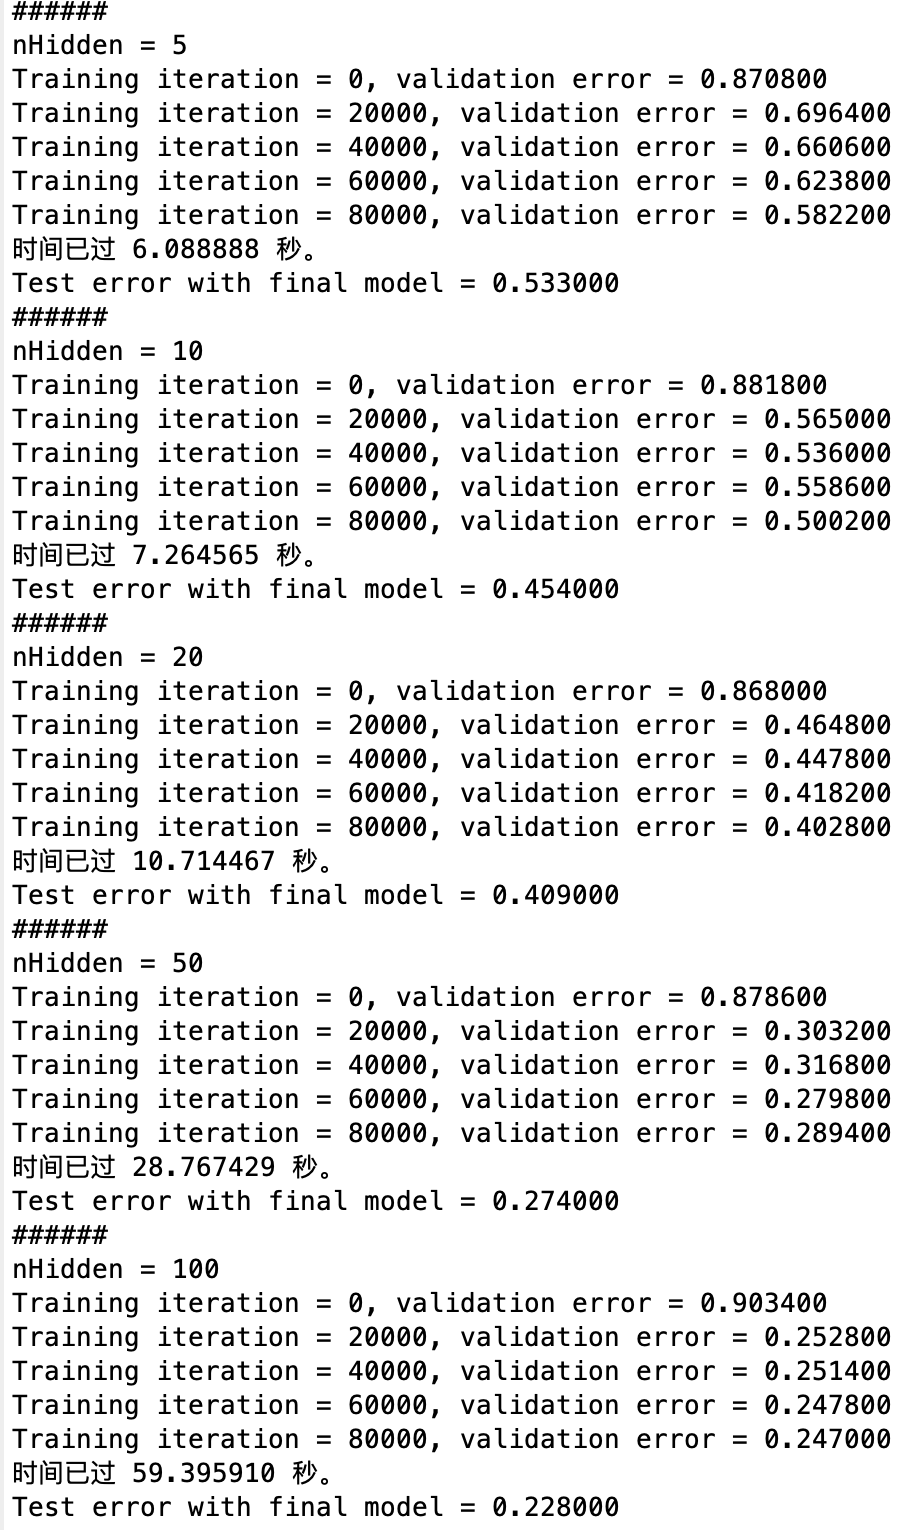
\includegraphics[width=0.5\linewidth]{figures/q1-1.png}
  \caption{Different \textit{nHidden}, single hidden layer}
  \label{fig:q1-1}
\end{figure}

\begin{figure}[htbp]
  \centering
  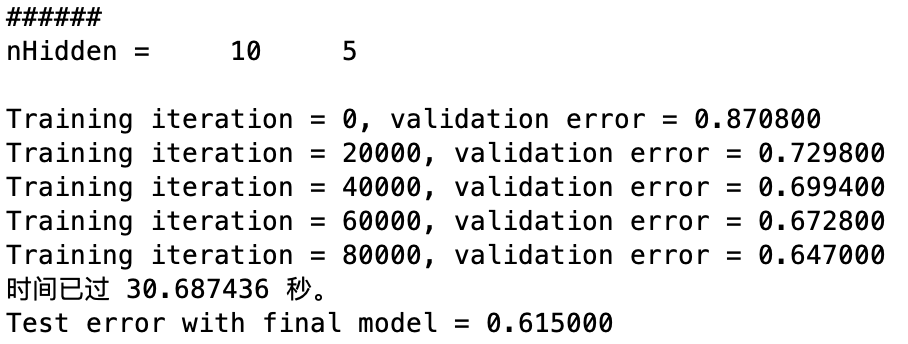
\includegraphics[width=0.5\linewidth]{figures/q1-2.png}
  \caption{Two hidden layers}
  \label{fig:q1-2}
\end{figure}

(code in \texttt{q1.m})

\autoref{fig:q1-1} shows model performances with different number of hidden units and a single hidden layer. We can see that test accuracy increases as \textit{nHidden} increases, but a larger moel requires longer training time. \autoref{fig:q1-2} shows model performance with two hidden layers. The two-layer model's performance is even worse than that of a single-layer model, and it also takes a longer training time. We may infer that, in this simple digit classification problem, model with a single hidden layer is good enough to represent the features of the images. 


\item Change the training procedure by modifying the sequence of step-sizes or using different step-sizes for different variables. That momentum uses the update
$$
w^{t+1} = w^t - \alpha_t \nabla f(w^t) + \beta^t (w^t - w^{t-1})
$$
where $\alpha_t$ is the learning rate (step size) and $\beta_t$ is the momentum strength. A common value of $\beta_t$ is a constant 0.9.

\begin{figure}[htbp]
  \centering
  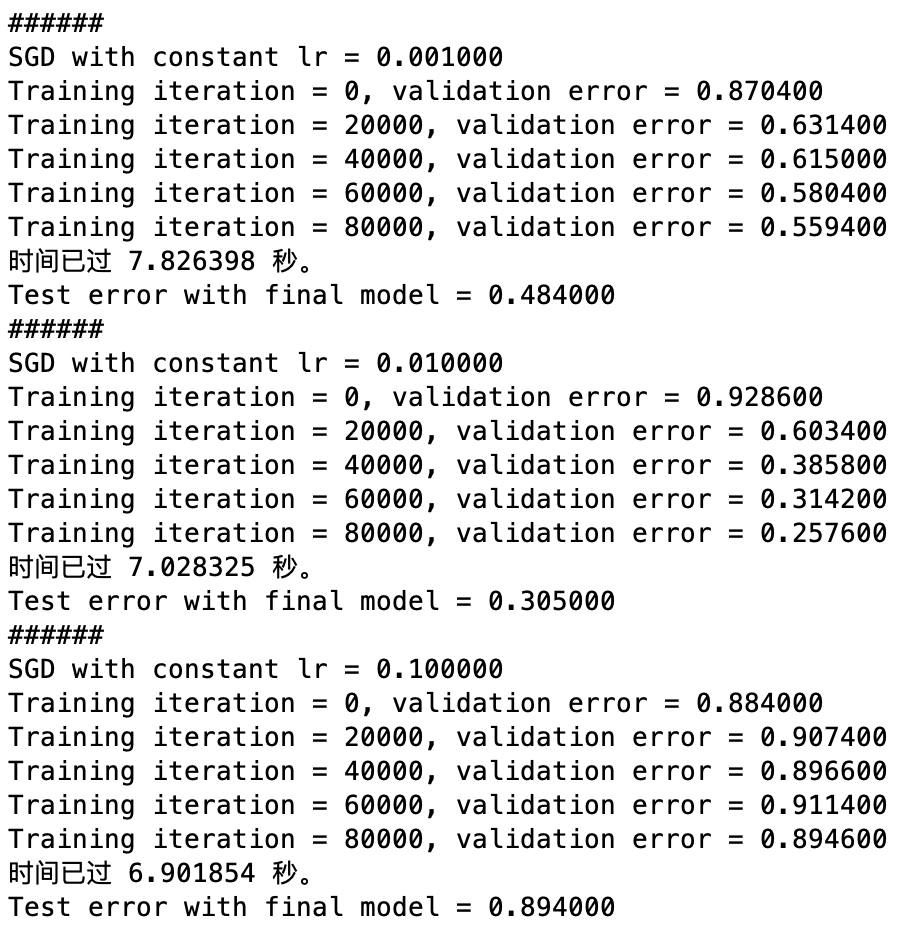
\includegraphics[width=0.5\linewidth]{figures/q2-1.png}
  \caption{SGD with different constant learning rates}
  \label{fig:q2-1}
\end{figure}

\begin{figure}[htbp]
  \centering
  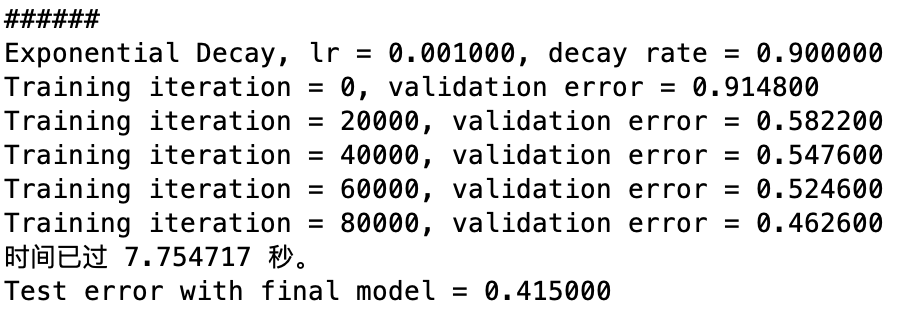
\includegraphics[width=0.5\linewidth]{figures/q2-2.png}
  \caption{Exponential decay learning rate}
  \label{fig:q2-2}
\end{figure}

\begin{figure}[htbp]
  \centering
  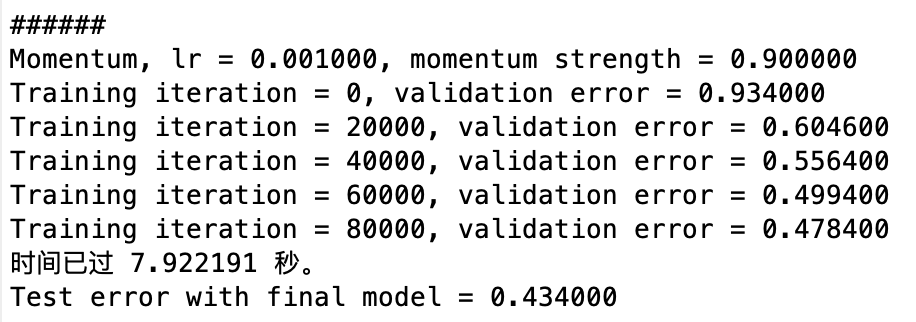
\includegraphics[width=0.5\linewidth]{figures/q2-3.png}
  \caption{Momentum}
  \label{fig:q2-3}
\end{figure}

(code in \texttt{q2.m})

\autoref{fig:q2-1}, \autoref{fig:q2-2}, \autoref{fig:q2-3} shows model perfromances of stochastic gradient descend (SGD) with constant learning rate (lr), SGD with exponential decay lr, and momentum method, all with $nHidden = 10$. We can see from \autoref{fig:q2-1} that, with a constant lr of 0.01 or 0.001, the model successfully learned something; but with a large constant lr of 0.1, the model failed to converge. Besides, by comparing \autoref{fig:q2-1}, \autoref{fig:q2-2} and \autoref{fig:q2-3}, we can see that both SGD with exponential decay lr and momentum have higher accuracy than SGD with constant lr. 

\item You could vectorize evaluating the loss function (e.g., try to express as much as possible in terms of matrix operations), to allow you to do more training iterations in a reasonable amount of time.

\begin{figure}[htbp]
  \centering
  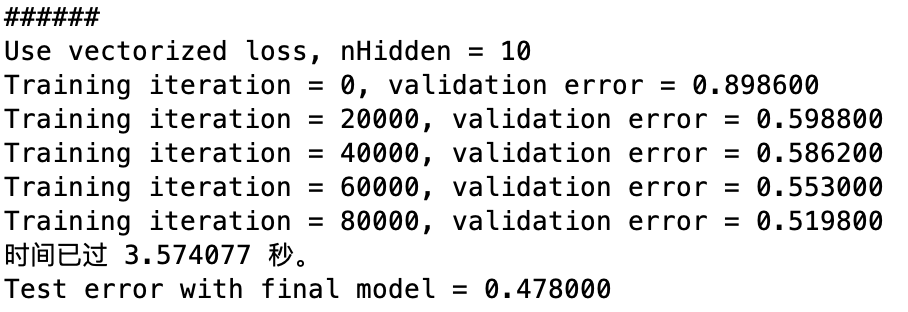
\includegraphics[width=0.5\linewidth]{figures/q3-1.png}
  \caption{Vectorized loss, single hidden layer}
  \label{fig:q3-1}
\end{figure}

\begin{figure}[htbp]
  \centering
  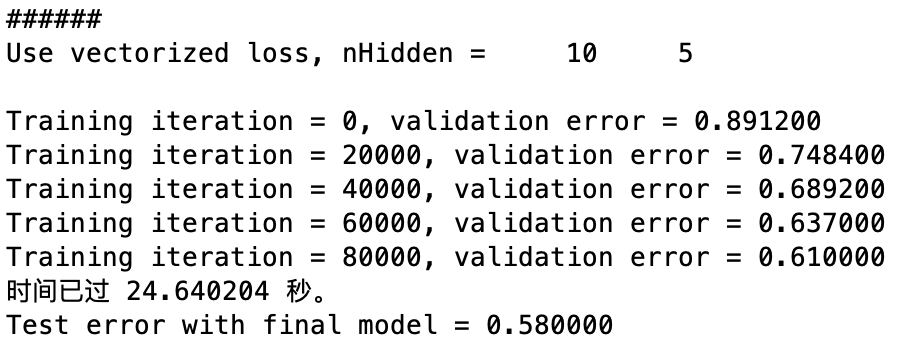
\includegraphics[width=0.5\linewidth]{figures/q3-2.png}
  \caption{Vectorized loss, two hidden layers}
  \label{fig:q3-2}
\end{figure}

(code in \texttt{q3.m} and \texttt{q3\_vectirized\_MLPLoss.m})

\autoref{fig:q3-1} and \autoref{fig:q3-2} shows model results with vectorized loss function (lr=0.001). In this way, training time can be saved without loss of model performance.

\item Add $l_2$-regularization (or $l_1$-regularization) of the weights to your loss function. For neural networks this is called \textit{weight decay}. An alternate form of regularization that is sometimes used is \textit{early stopping}, which is stopping training when the error on a validation set stops decreasing.

\begin{figure}[htbp]
  \centering
  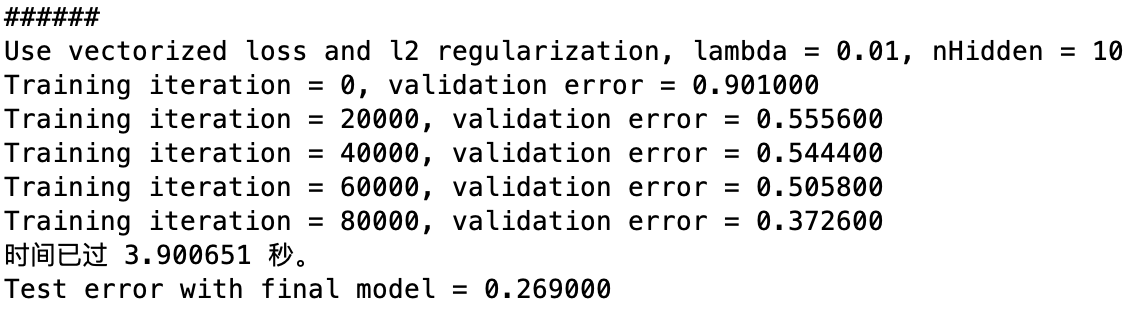
\includegraphics[width=0.5\linewidth]{figures/q4-1.png}
  \caption{$l_2$-regularization, single hidden layer}
  \label{fig:q4-1}
\end{figure}

\begin{figure}[htbp]
  \centering
  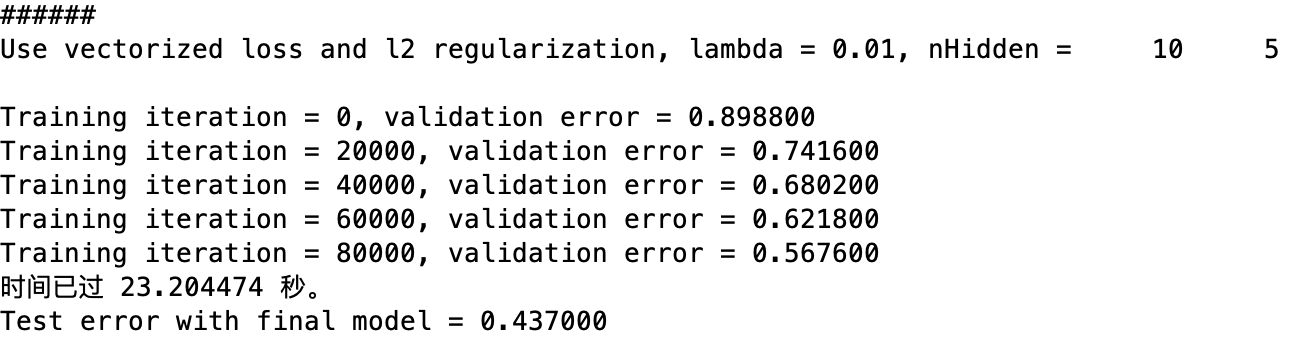
\includegraphics[width=0.5\linewidth]{figures/q4-2.png}
  \caption{$l_2$-regularization, two hidden layers}
  \label{fig:q4-2}
\end{figure}

(code in \texttt{q4.m})

Results are shown in \autoref{fig:q4-1} and \autoref{fig:q4-2} (lr=0.001). We can see that $l_2$-regularization improves model performance. The reason may be that over-parameterization can be avoided through this approach.

\item Instead of using the squared error, use a softmax (multinomial logistic) layer at the end of the network so that the 10 outputs can be interpreted as probabilities of each class. Recall that the softmax function is
$$
p(y_i) = \frac{\exp(z_i)}{\sum_{j=1}^J\exp(z_j)}
$$
you can replace squared error with the negative log-likelihood of the true label under this loss, $-\log p(y_i)$.

\begin{figure}[htbp]
  \centering
  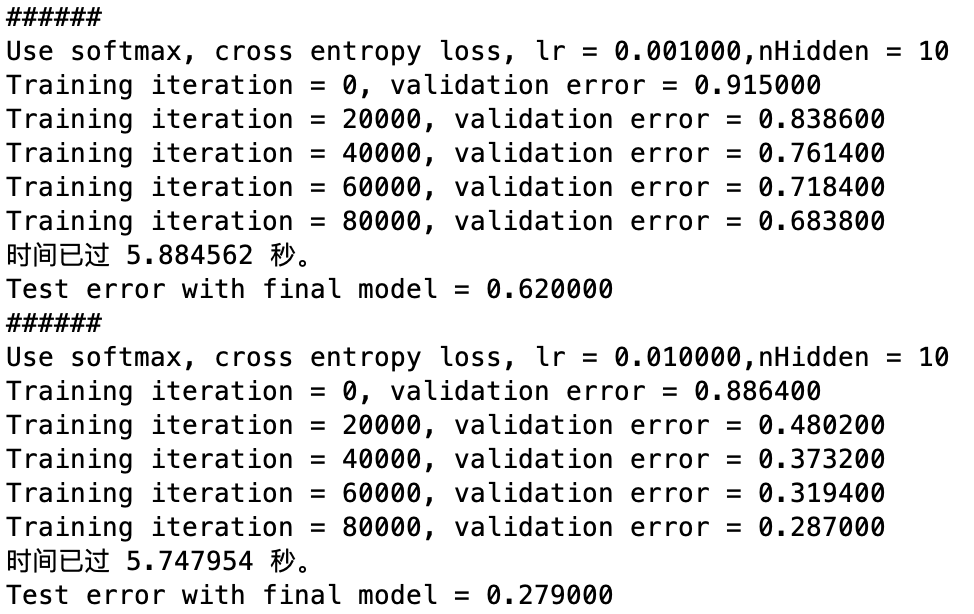
\includegraphics[width=0.5\linewidth]{figures/q5-1.png}
  \caption{softmax, single hidden layer}
  \label{fig:q5-1}
\end{figure}

\begin{figure}[htbp]
  \centering
  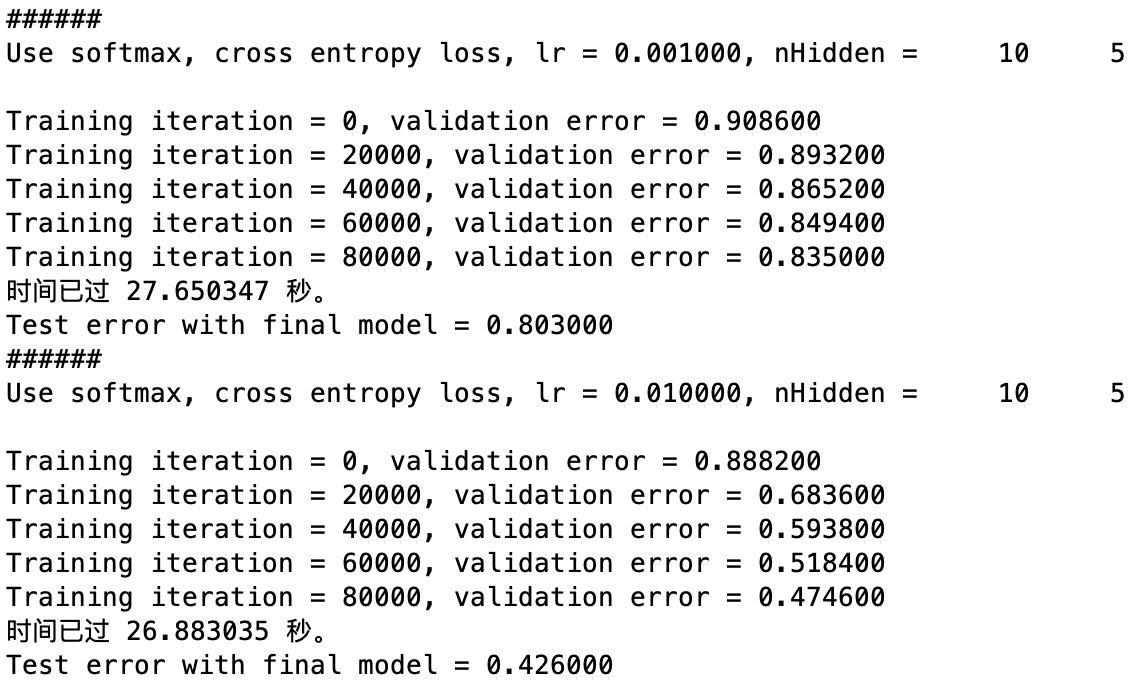
\includegraphics[width=0.5\linewidth]{figures/q5-2.png}
  \caption{softmax, two hidden layers}
  \label{fig:q5-2}
\end{figure}

(code in \texttt{q5.m} and \texttt{q5\_CE\_MLPLoss.m})

Results are shown in \autoref{fig:q5-1} and \autoref{fig:q5-2}. With a softmax layer, the model performance improves with a small increase in training time. Besides, the learning rate should be adjusted to fit the new model.

\item Instead of just having a bias variable at the beginning, make one of the hidden units in each layer a constant, so that each layer has a bias.

\begin{figure}[htbp]
  \centering
  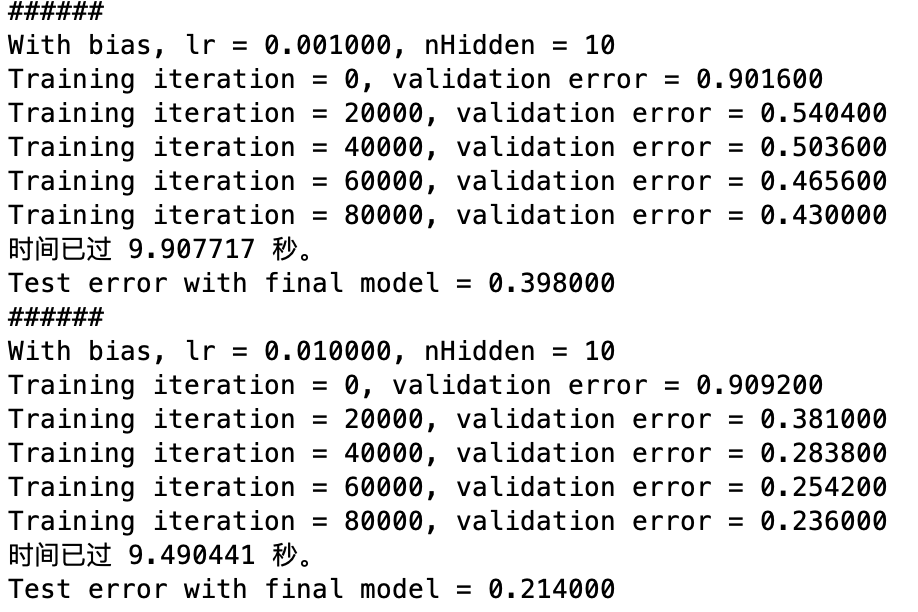
\includegraphics[width=0.5\linewidth]{figures/q6-1.png}
  \caption{with bias, single hidden layer}
  \label{fig:q6-1}
\end{figure}

\begin{figure}[htbp]
  \centering
  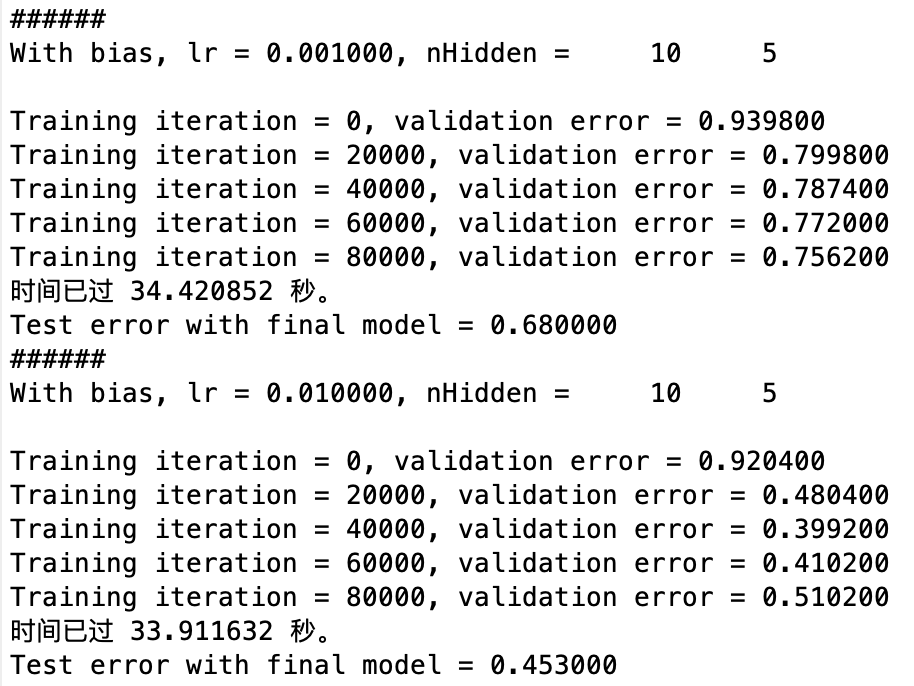
\includegraphics[width=0.5\linewidth]{figures/q6-2.png}
  \caption{with bias, two hidden layers}
  \label{fig:q6-2}
\end{figure}

(code in \texttt{q6.m}, \texttt{q6\_MLP\_with\_bias.m}, and \texttt{q6\_Predict\_with\_bias.m})

Results are shown in \autoref{fig:q6-1} and \autoref{fig:q6-2}. The model performances are improved with bias, with increased training time. The lr also needs to be tuned.

\item Implement ``dropout'', in which hidden units are dropped out with probability $p$ during training. A common choice is $p = 0.5$.

\begin{figure}[htbp]
  \centering
  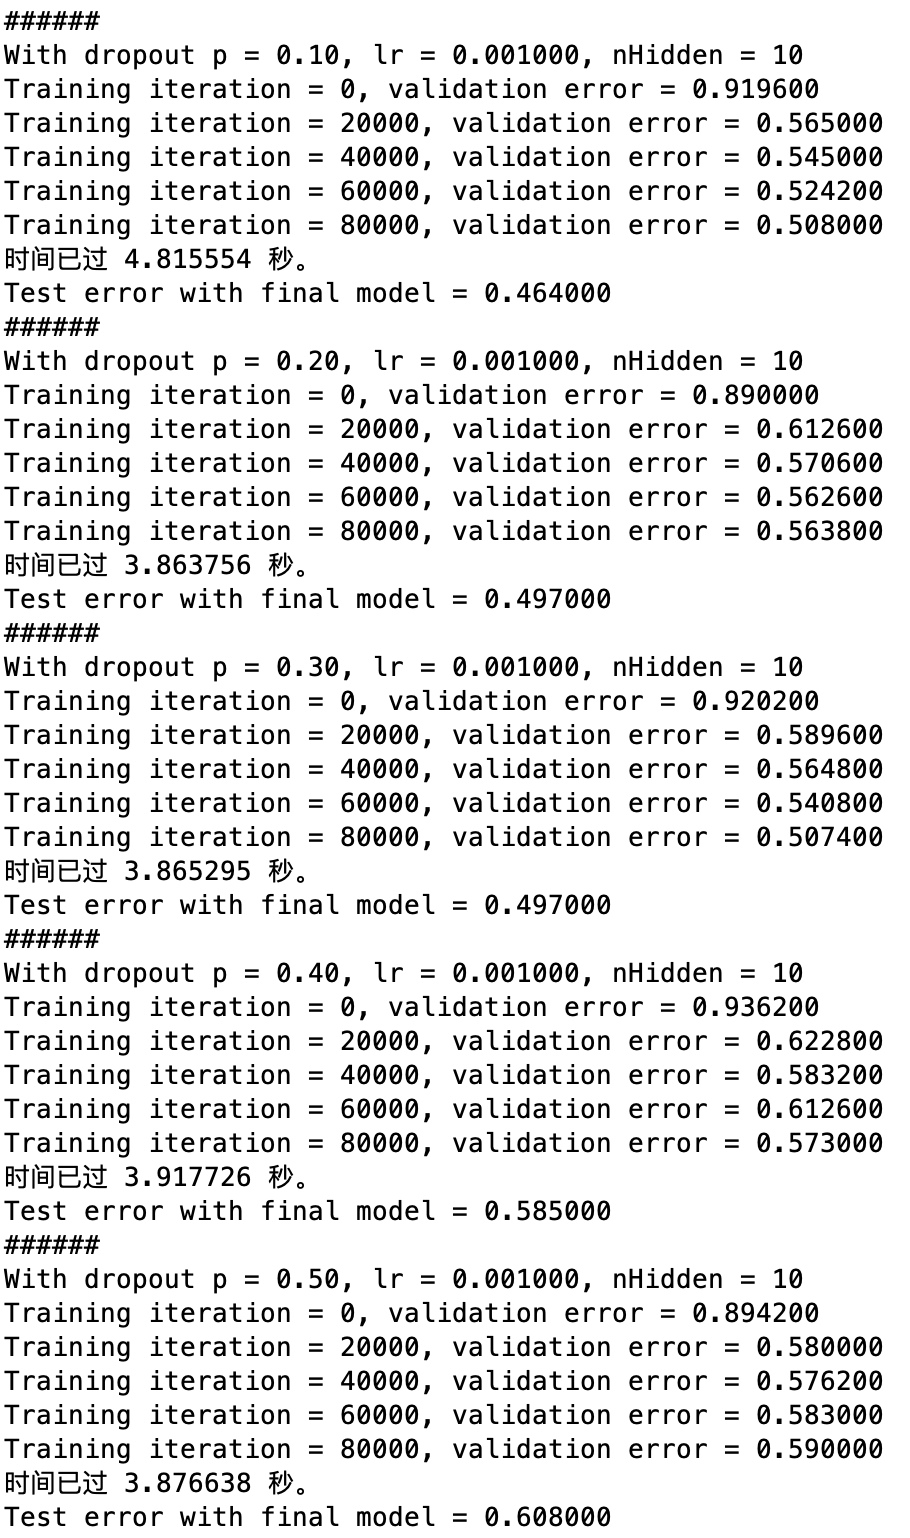
\includegraphics[width=0.5\linewidth]{figures/q7-1.png}
  \caption{with dropout, different $p$}
  \label{fig:q7-1}
\end{figure}

(code in \texttt{q7.m} and \texttt{q7\_MLP\_with\_dropout.m})

Results are shown in \autoref{fig:q7-1}, with $p\in(0.1,0.2,0.3,0.4,0.5)$ tested. We can see that the model performance decreases as $p$ increases. The reason may be that the model is relatively small (with $nHidden=10$), so every neuron is somehow important in the hidden layer. 

\item You can do 'fine-tuning' of the last layer. Fix the parameters of all the layers except the last one, and solve for the parameters of the last layer exactly as a convex optimization problem. E.g., treat the input to the last layer as the features and use techniques from earlier in the course (this is particularly fast if you use the squared error, since it has a closed-form solution).

\begin{figure}[htbp]
  \centering
  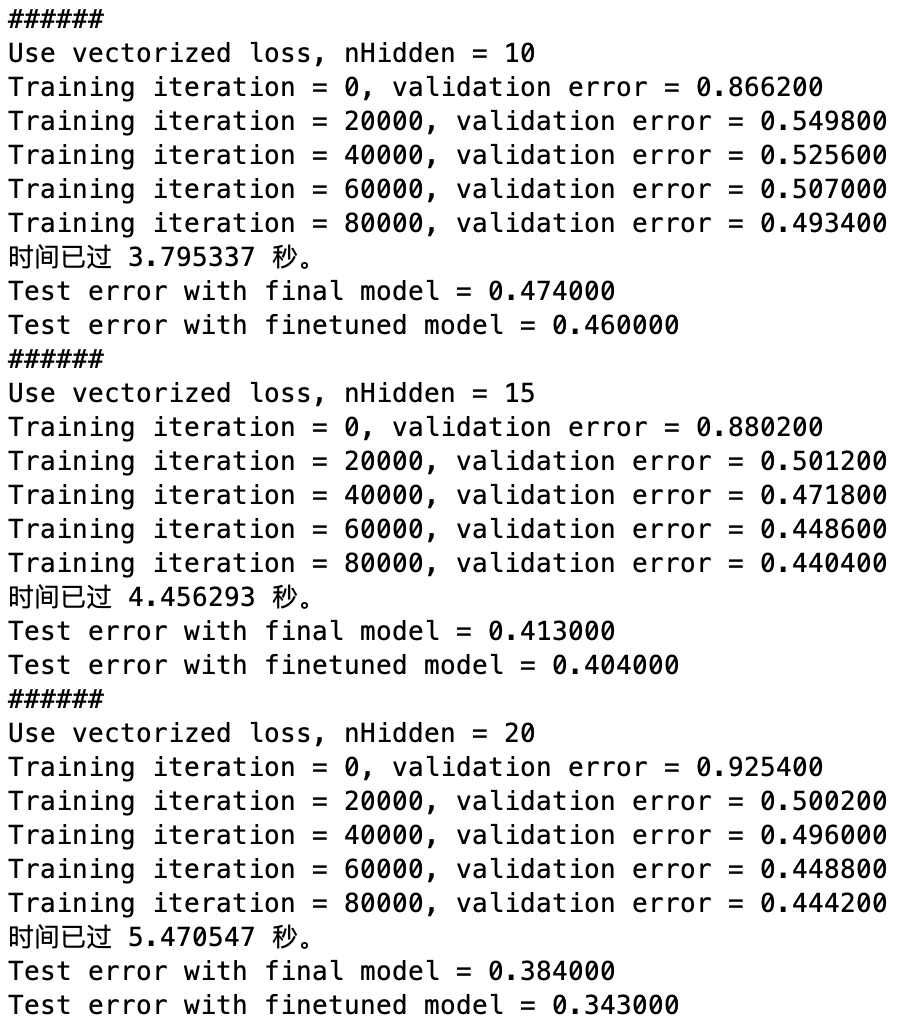
\includegraphics[width=0.5\linewidth]{figures/q8-1.png}
  \caption{with fine-tuning}
  \label{fig:q8-1}
\end{figure}

(code in \texttt{q8.m} and \texttt{q8\_Predict\_finetune.m})

Results are shown in \autoref{fig:q8-1}, with $nHidden\in(10,15,20)$. We can see that the model performance slightly improves if we use the finetuning method.

\item You can artificially create more training examples, by applying small transformations (translations, rotations, resizing, etc.) to the original images.

\begin{figure}[htbp]
  \centering
  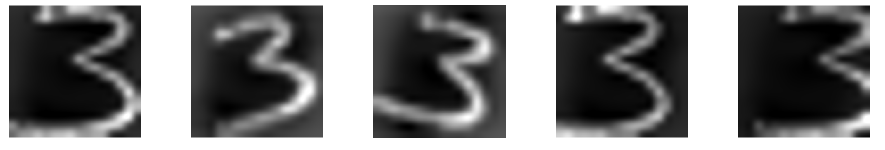
\includegraphics[width=0.8\linewidth]{figures/digits.png}
  \caption{data augmentation example}
  \label{fig:digits}
\end{figure}

\begin{figure}[htbp]
  \centering
  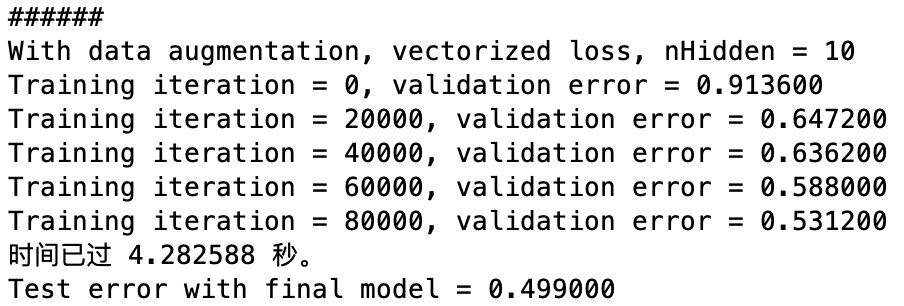
\includegraphics[width=0.5\linewidth]{figures/q9-1.png}
  \caption{with data augmentation}
  \label{fig:q9-1}
\end{figure}

(code in \texttt{q9.m}, \texttt{data\_augmentation.m} and \texttt{visualize\_image.m})

I implemented data augmentation by applying small rotations and moves to the original images. An example is shown in \autoref{fig:digits} (from left to right: original, rotate $15^\circ$ anti-clockwise, rotate $15^\circ$ clockwise, move 2 pixels to the left, move 2 pixels to the right). 

Model result trained with data augmentation is shown in \autoref{fig:q9-1}. Surprisingly, there is no observable difference between augmented or not-augmented model. The reason may be that the task is relatively simple (with a small image), so the original data is enough for training.

\item Replace the first layer of the network with a 2D convolutional layer. You will need to reshape the USPS images back to their original 16 by 16 format. The Matlab conv2 function implements 2D convolutions. Filters of size 5 by 5 are a common choice.

\begin{figure}[htbp]
  \centering
  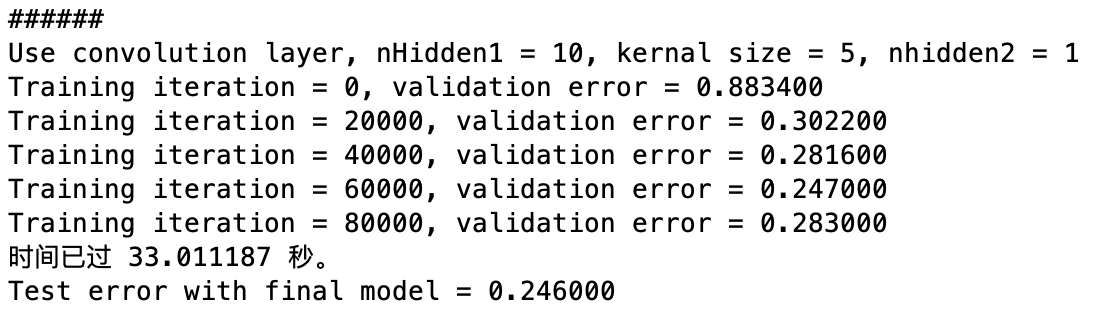
\includegraphics[width=0.5\linewidth]{figures/q10-1.png}
  \caption{with convolution layer}
  \label{fig:q10-1}
\end{figure}

(code in \texttt{q10.m}, \texttt{ConvNet.m} and \texttt{Conv\_Predict.m})

\autoref{fig:q10-1} shows the result of model with a convolution layer, with kernal size 5. Training time increases dramatically, but the model performance also improves greatly. 

\end{enumerate}

\subsection{Final Model}

(code in \texttt{final\_model.m})

The final model uses 4 convolution layers with kernel size 3, followed by three full-connected layers of size $[128, 64, 32]$, model result is shown in \autoref{fig:final-1}.

The final model uses the trick of Xavier initialization \footnote{Glorot, X., \& Bengio, Y. (2010, March). Understanding the difficulty of training deep feedforward neural networks. In \textit{Proceedings of the thirteenth international conference on artificial intelligence and statistics} (pp. 249-256). JMLR Workshop and Conference Proceedings.}, which can greatly accelerate the training process. As a comparison, if we train the model without Xavier initialization, the model converges much slower and fails to achieve a good performance after the same number of iterations, as shown in \autoref{fig:final-2} and \autoref{fig:final-plot-1}.

If the FC layers are removed, training time reduces by half, but model performances become worse, and Xavier initialization trick still helps, as shown in \autoref{fig:final-3}, \autoref{fig:final-4} and \autoref{fig:final-plot-2}.

\begin{figure}[htbp]
  \centering
  \begin{minipage}{0.48\linewidth}
    \centering
    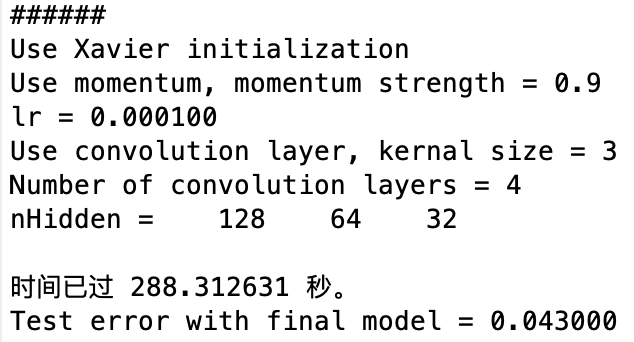
\includegraphics[width=\linewidth]{figures/final-1.png}
    \caption{the final model}
    \label{fig:final-1}
  \end{minipage}
  \begin{minipage}{0.48\linewidth}
    \centering
    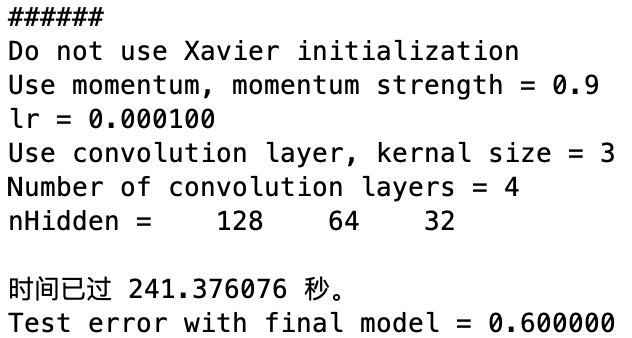
\includegraphics[width=\linewidth]{figures/final-2.png}
    \caption{compare model A}
    \label{fig:final-2}
  \end{minipage}
\end{figure}

\begin{figure}[htbp]
  \centering
  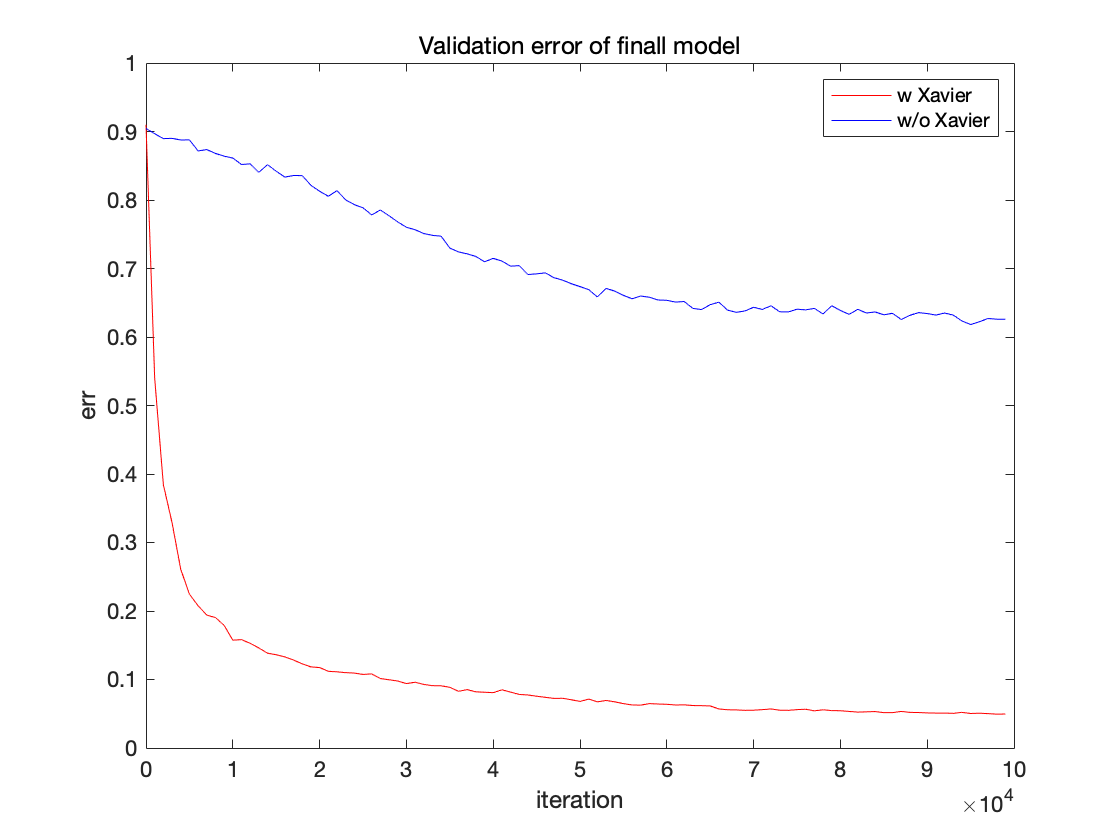
\includegraphics[width=0.8\linewidth]{figures/final-plot-1.png}
  \caption{comparison w and w/o Xavier, with FC layers}
  \label{fig:final-plot-1}
\end{figure}

\begin{figure}[htbp]
  \centering
  \begin{minipage}{0.48\linewidth}
    \centering
    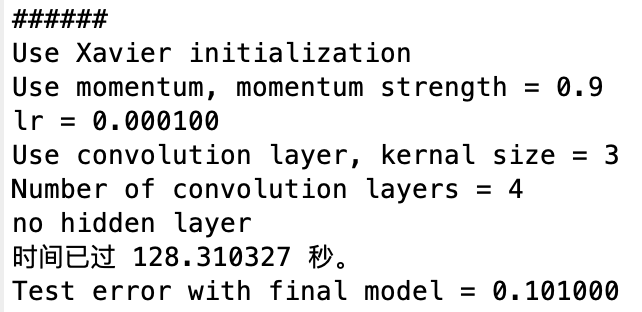
\includegraphics[width=\linewidth]{figures/final-3.png}
    \caption{compare model B}
    \label{fig:final-3}
  \end{minipage}
  \begin{minipage}{0.48\linewidth}
    \centering
    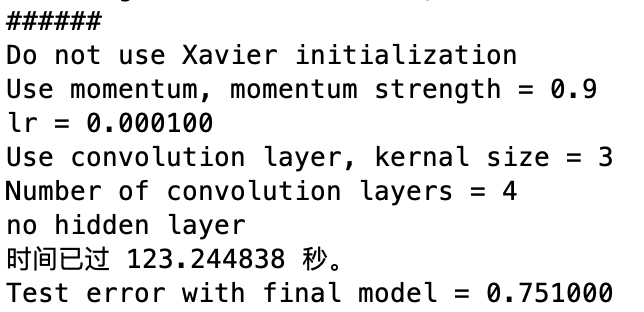
\includegraphics[width=\linewidth]{figures/final-4.png}
    \caption{compare model C}
    \label{fig:final-4}
  \end{minipage}
\end{figure}

\begin{figure}[htbp]
  \centering
  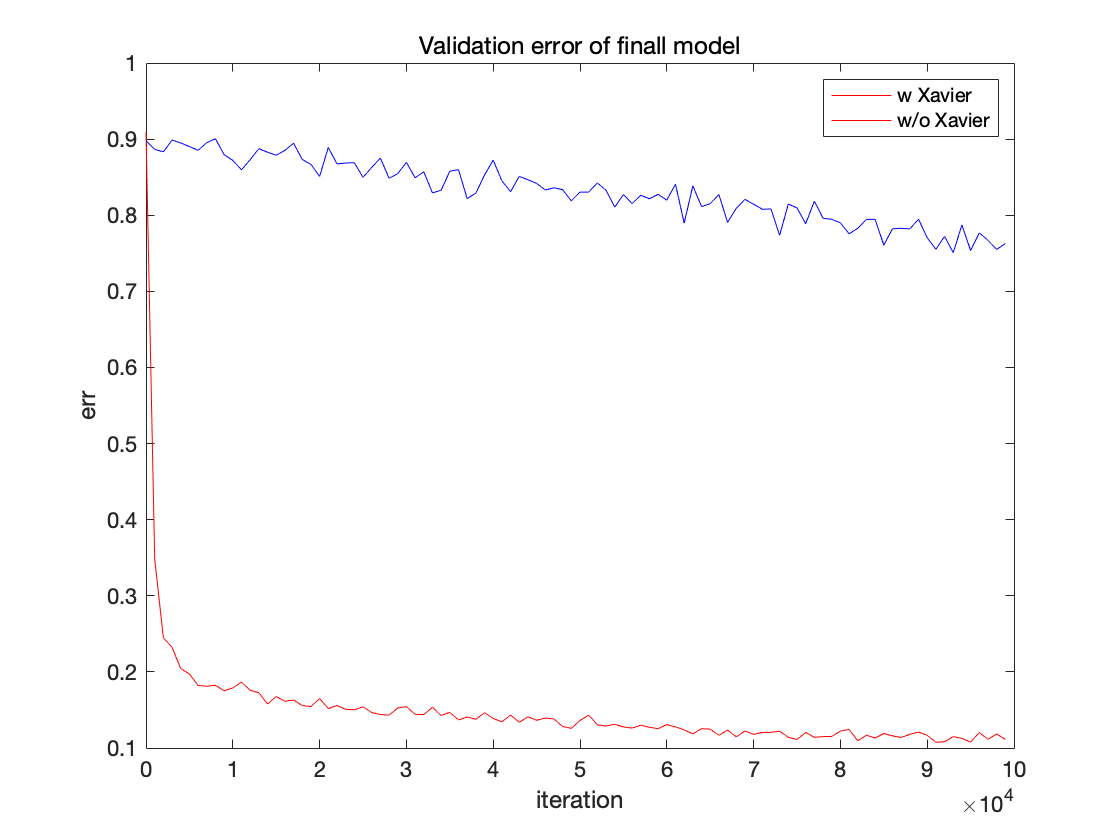
\includegraphics[width=0.8\linewidth]{figures/final-plot-2.png}
  \caption{comparison w and w/o Xavier, w/o FC layers}
  \label{fig:final-plot-2}
\end{figure}


%-------------------------------------
%=====================
%\bibliographystyle{plain}
%\interlinepenalty=10000
%\bibliography{reference}

\end{document}
